\documentclass[a4paper]{article}

\usepackage[english]{babel}
\usepackage[utf8]{inputenc}
\usepackage{amsmath}
\usepackage{float}
\usepackage{graphicx}
\usepackage[colorinlistoftodos]{todonotes}

\usepackage{geometry}
 \geometry{
 a4paper,
 total={170mm,257mm},
 left=20mm,
 top=20mm,
 }
 
\title{Report \#2}

\author{Ariel Soto Caro}

\date{\today}

\begin{document}
\maketitle

\section{Pooled estimation}
Table 1 shows the summary of OLS models. Figures 1 and 2 compares the model with a trend and a dummy per year.

\begin{table}[H]
  \centering
  \caption{NEW Summary of SFA regressions}
  \scalebox{1.0}{
    \begin{tabular}{lrrrrrrrr} \hline
          & \multicolumn{4}{c}{PRODUCTION} & \multicolumn{4}{c}{COST} \\ \hline
    \textit{Coefficient} & \multicolumn{2}{c}{\textit{with trend}} & \multicolumn{2}{c}{\textit{dummy per year}} & \multicolumn{2}{c}{\textit{with trend}} & \multicolumn{2}{c}{\textit{dummy per year}} \\ \hline \hline
    (Intercept) & 5.071 & \multicolumn{1}{l}{***} & 5.031 & \multicolumn{1}{l}{***} & -2.470 & \multicolumn{1}{l}{***} & -2.208 & \multicolumn{1}{l}{***} \\
    log(output) &       &       &       &       & 0.937 & \multicolumn{1}{l}{***}     & 0.937 & \multicolumn{1}{l}{***} \\
    log(labor) & 0.192 & \multicolumn{1}{l}{***} & 0.193 & \multicolumn{1}{l}{***} & 0.036 & \multicolumn{1}{l}{***} & 0.046 & \multicolumn{1}{l}{***} \\
    log(fuel) & 0.625 & \multicolumn{1}{l}{***} & 0.625 & \multicolumn{1}{l}{***} & 0.372 & \multicolumn{1}{l}{} & 0.369 & \multicolumn{1}{l}{} \\
    log(capital) & 0.174 & \multicolumn{1}{l}{***} & 0.173 & \multicolumn{1}{l}{***} & 0.481 & \multicolumn{1}{l}{***} & 0.590 & \multicolumn{1}{l}{***} \\
    trend & 0.015 & \multicolumn{1}{l}{***} &       &       & -0.024 & \multicolumn{1}{l}{***} &       & \multicolumn{1}{l}{***} \\
    year87 &       &       & 0.089 & \multicolumn{1}{l}{*} &       &       & -0.089 & \multicolumn{1}{l}{*} \\
    year88 &       &       & 0.090 & \multicolumn{1}{l}{*} &       &       & -0.162 & \multicolumn{1}{l}{***} \\
    year89 &       &       & 0.145 & \multicolumn{1}{l}{**} &       &       & -0.190 & \multicolumn{1}{l}{***} \\
    year90 &       &       & 0.147 & \multicolumn{1}{l}{**} &       &       & -0.185 & \multicolumn{1}{l}{***} \\
    year91 &       &       & 0.142 & \multicolumn{1}{l}{***} &       &       & -0.204 & \multicolumn{1}{l}{***} \\
    year92 &       &       & 0.141 & \multicolumn{1}{l}{***} &       &       & -0.200 & \multicolumn{1}{l}{***} \\
    year93 &       &       & 0.118 & \multicolumn{1}{l}{***} &       &       & -0.171 & \multicolumn{1}{l}{***} \\
    year94 &       &       & 0.155 & \multicolumn{1}{l}{***} &       &       & -0.268 & \multicolumn{1}{l}{***} \\
    year95 &       &       & 0.178 & \multicolumn{1}{l}{***} &       &       & -0.292 & \multicolumn{1}{l}{***} \\
    year96 &       &       & 0.225 & \multicolumn{1}{l}{***} &       &       & -0.304 & \multicolumn{1}{l}{***} \\ \hline
    $R^2$  & 0.933 &       & 0.934 &       & 0.938 &       & 0.939 &  \\ \hline
    \end{tabular}%
    }
  \label{tab2}%
\end{table}%


\newpage


\begin{figure}[H]
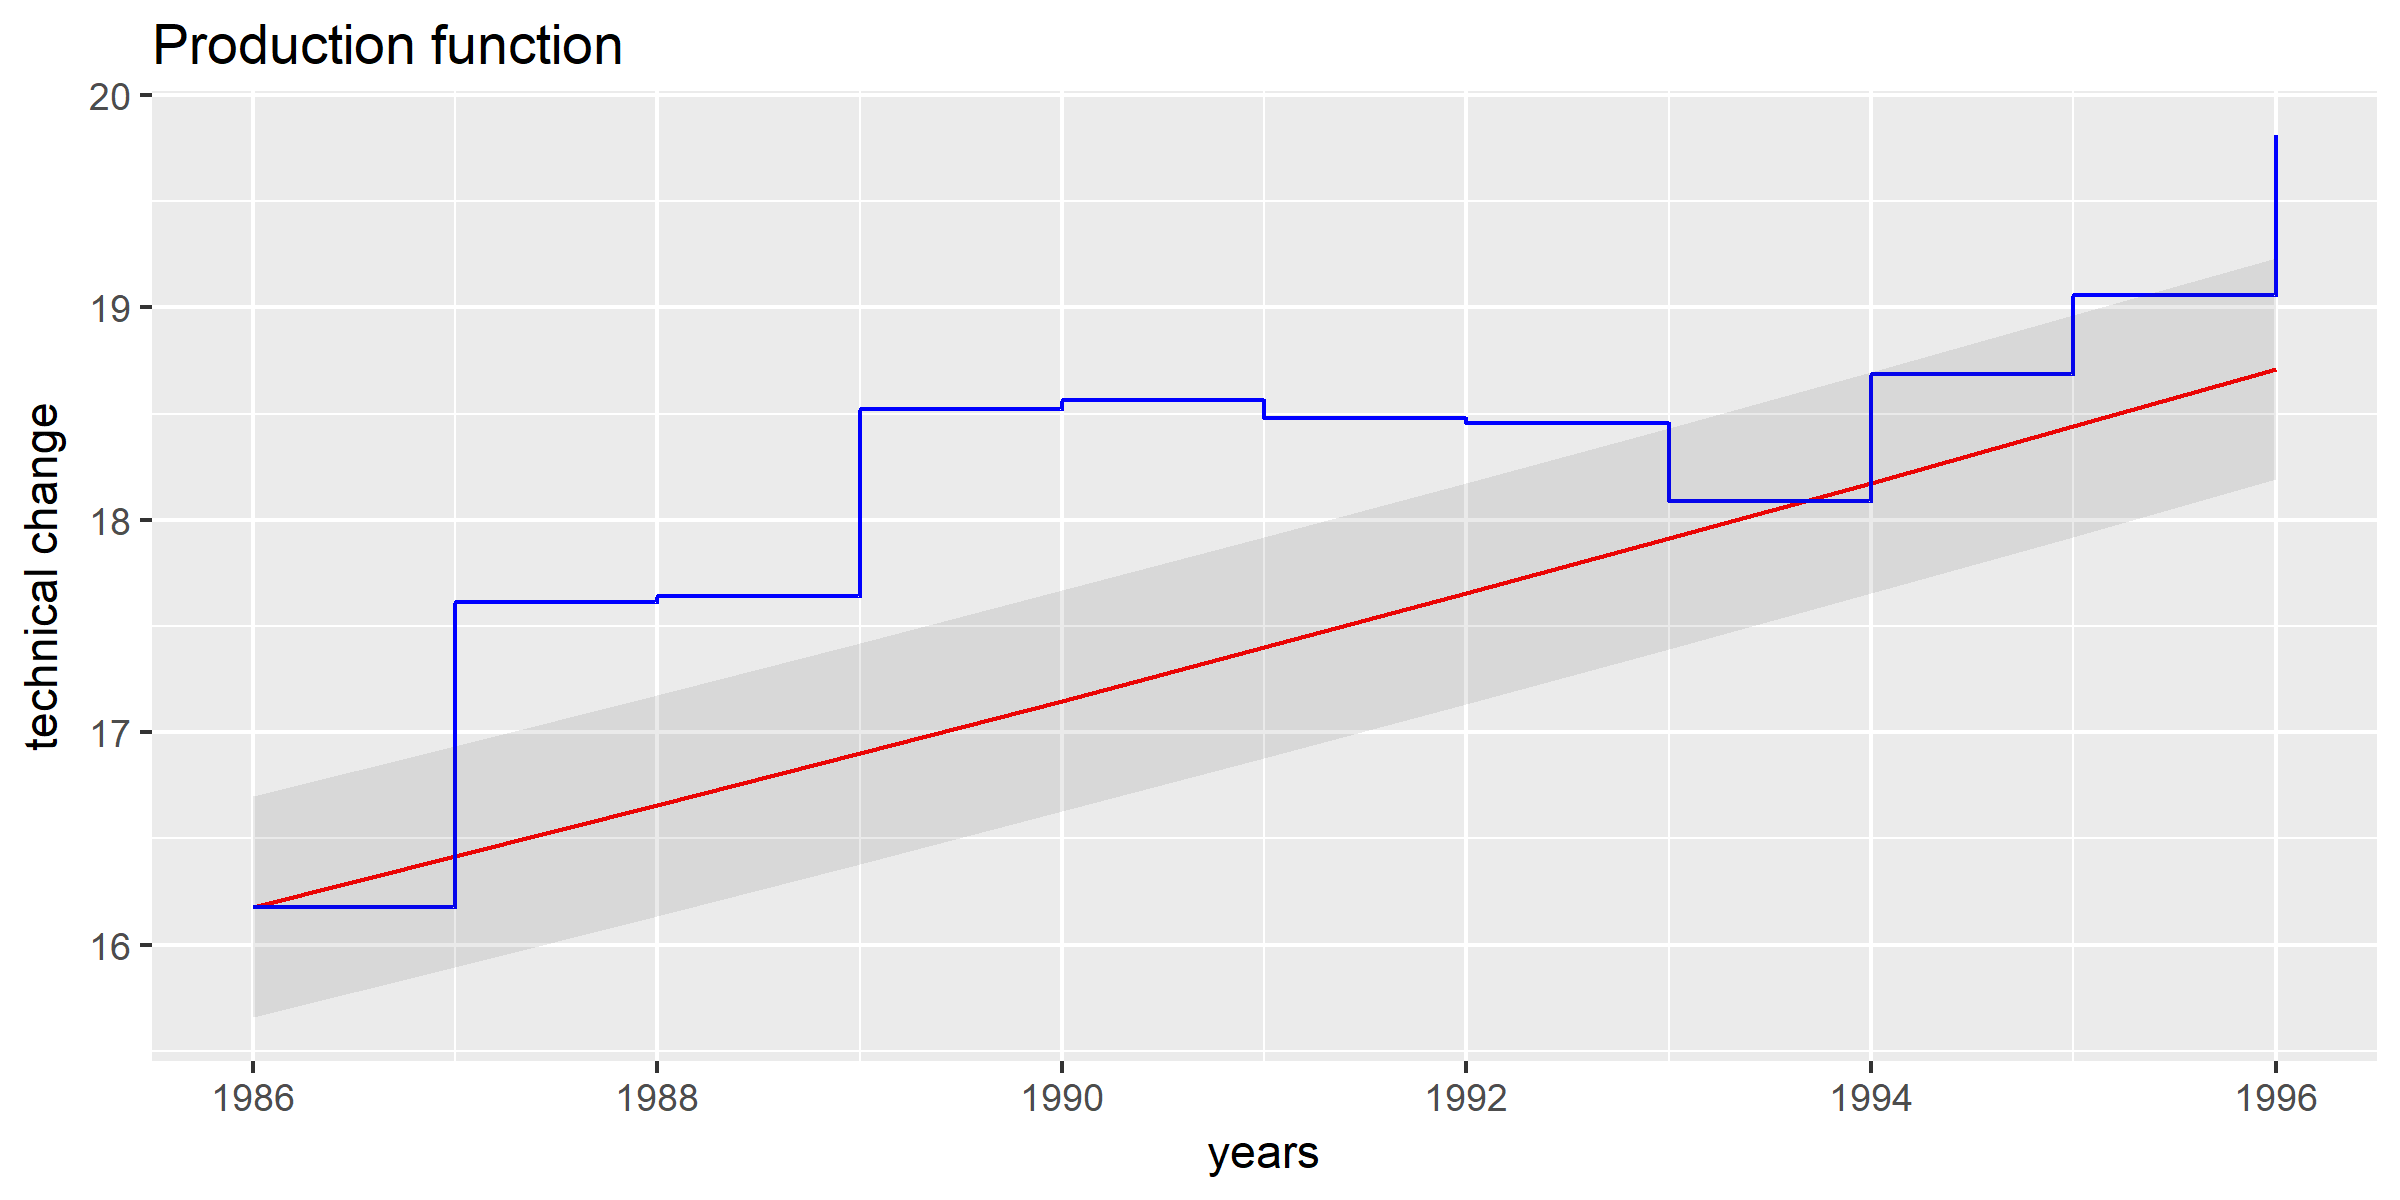
\includegraphics[scale=.90]{Prod_ols}
\end{figure}

\begin{figure}[H]
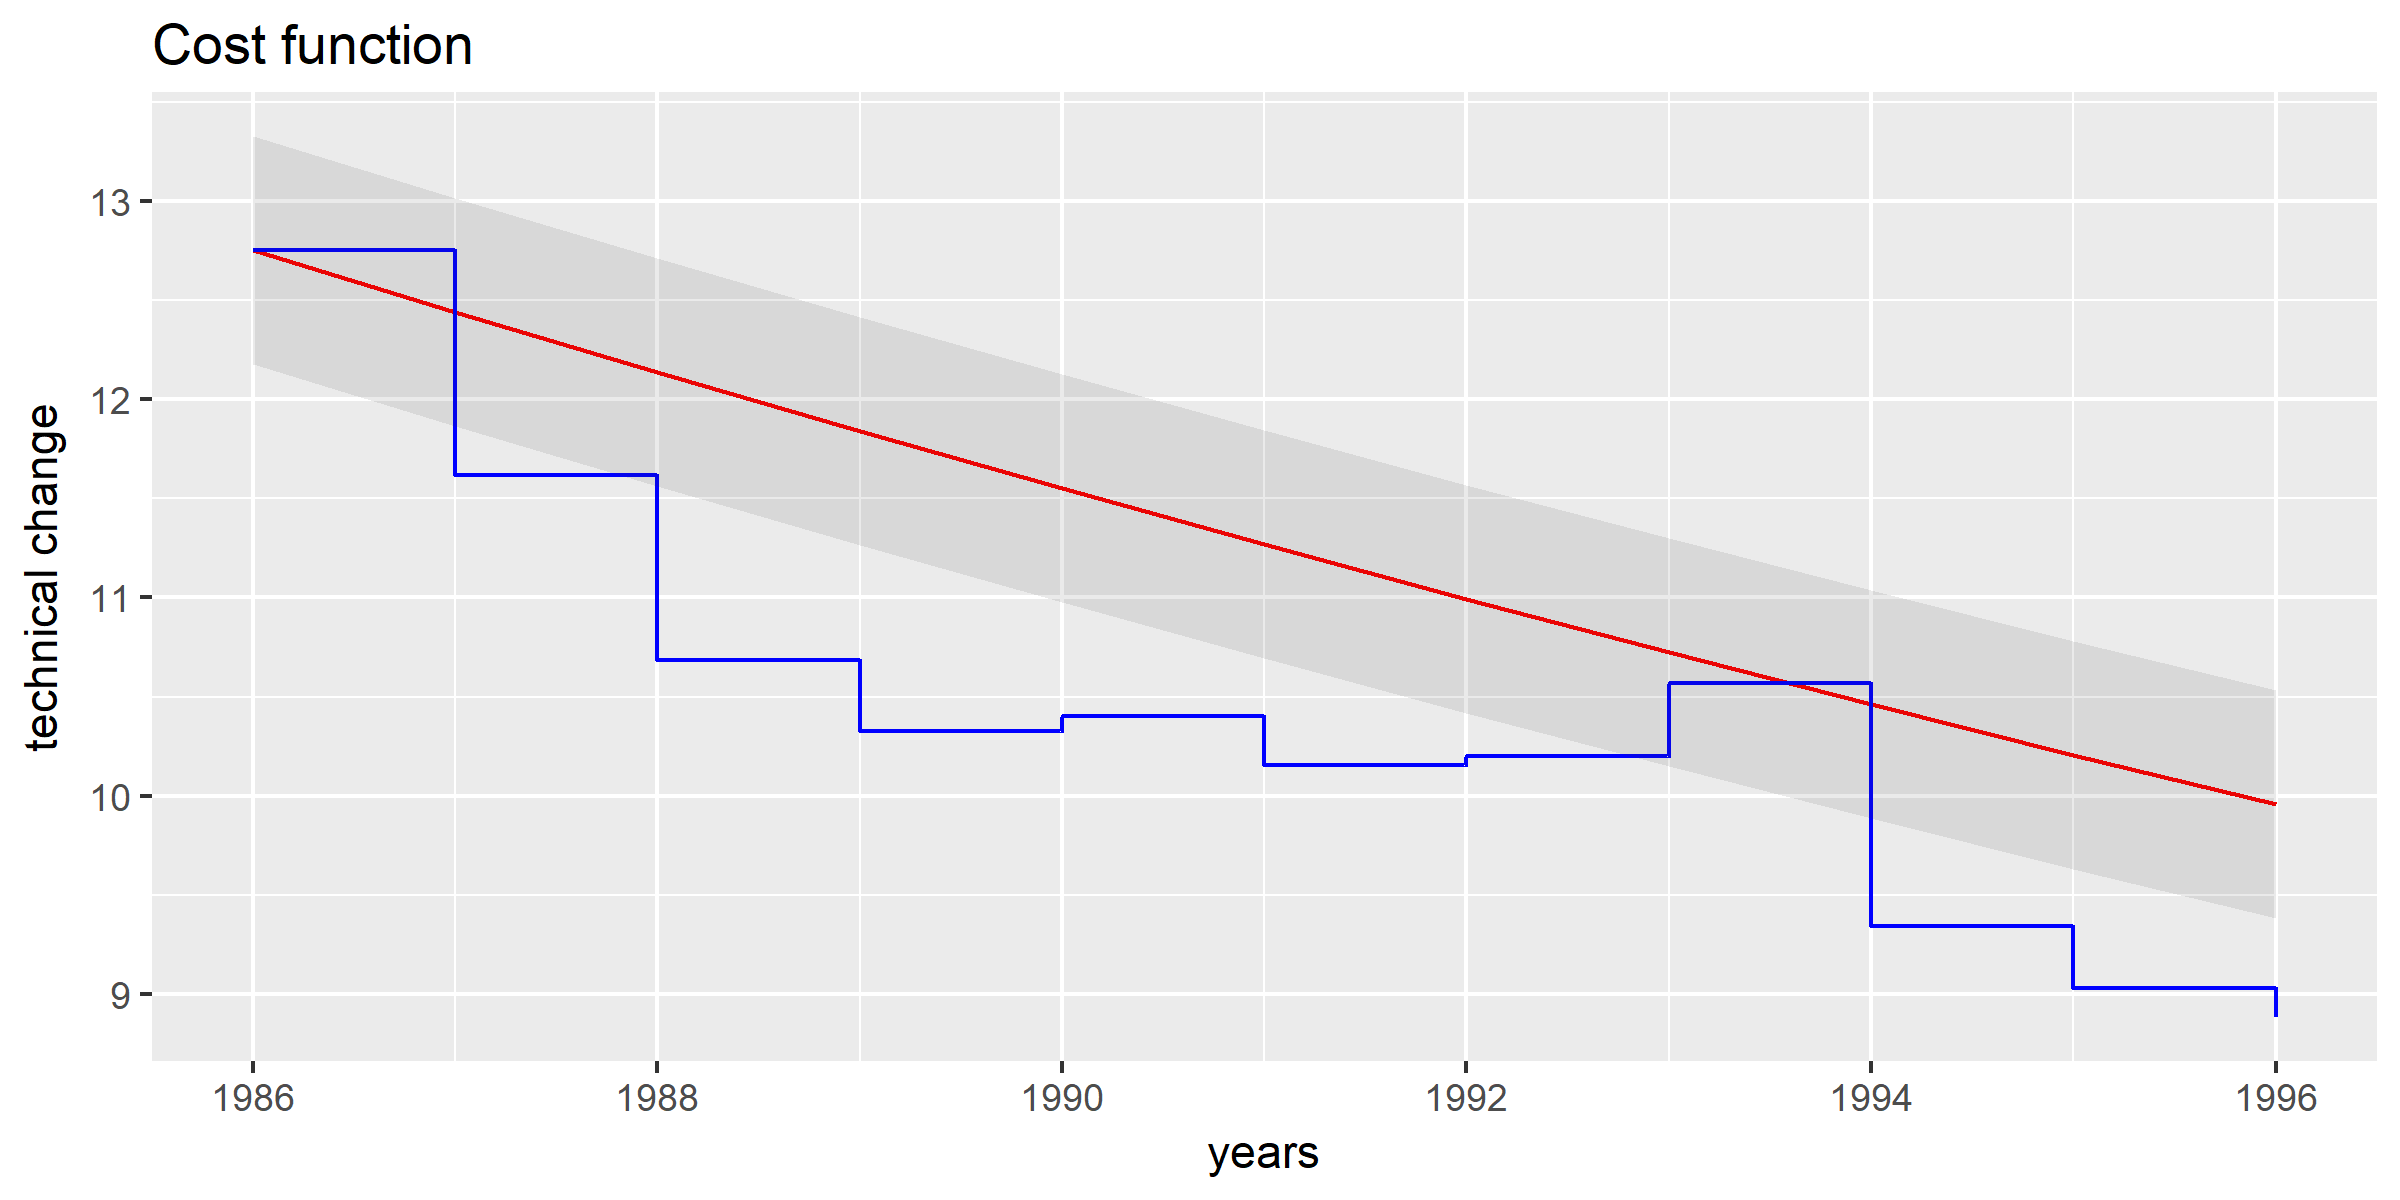
\includegraphics[scale=.90]{Cost_ols}
\end{figure}


\end{document}